%% Background chapter 
%% author Liu Peng 

Home networking has been a hot topic for quite a few years. Thanks to the rapid development 
of electronics and computer science, home networking devices are becoming more affordable 
and more powerful than they ever were. It is now so common that a person would have several multimedia devices that can be connected to the network. In this chapter, we give an overview of current solutions of home networking that bridges these multimedia devices. By making comparison among these solutions we try to identify the challenges that face home networking. 

\subsection{Overview} 
Early researches \cite{link_layer_old} \cite{end_user} \cite{link_layer} 
 conducted on home networking mainly aims to find out how home 
 networking infrastructures can be built. The subjects of these researches, including cable connection, wireless connection, optical connection etc, concerns more about the physical layer of the home network.  So far, it has turned out that the IEEE 802.11 protocol stack, among all others, is the most successful and  widely deployed home networking infrastructure. 

Nowadays, a typical scenario of home networking is that an IEEE 802.11 supportive wireless router connecting to a Ethernet cable or optical cable from the network operator creates a local network and other user devices simply join this network. The wireless Access Point(AP) employs the 802.11 b/g/n/ac protocol, utilizing the 2.4 GHz or 5 GHz frequency channels and providing a 100+ Mbps  network connection, whose bandwidth is sufficient for transmitting the popular High Definition (1080p) videos. 

In terms of network and application layer technologies, different device 
manufactures tend to choose their preferred multimedia-sharing protocols from the pool of protocols that have been evolving and developing for a long time.

Since late 1990s, UPnP protocol had been developed for home networking usage. 
At that time, XML was popular and widely used by different network applications.
Under such background, UPnP was designed to fully make use of XML. UPnP is 
independent of media types and devices and it runs on the TCP/IP stack, thus it can 
be easily applied to modern network infrastructures. 

In June 2003, Sony and several leading consumer electronic manufacturer s
established the Digital Living Network Alliance (DLNA), a nonprofit 
collaborative trade association. The DLNA standard is based on the widely used UPnP 
protocol but it added some restrictions on media formats and some compatibility 
requirements. A device hardware and software can be certified by DLNA 
organizations to prove that it can work with other devices that also passed 
this certification. 

In 2010, Apple quit DLNA and developed its own multimedia home networking 
solution, known as AirPlay. By adding screen mirroring, authentication and Remote 
Audio Output Protocol(RAOP) music streaming, Apple tried to forge a more advanced 
home network sharing system, aiming to provide a unique user experience among Apple 
products. Apple's solution had indeed attracted people's interest, and the user experience 
had proved much better than that of other similar products in the market. With its improvement
 over the years,  Apple's solution has now been acknowledged as one of the most popular streaming 
solutions .

Two years later, Wi-Fi alliance released its Miracast technology, and 
participated in pushing new standard in wireless home networking. The Miracast 
uses the Wi-Fi direct technology and it does not require a wireless local 
network. Instead, a peer-to-peer connection is created between the sharing and 
receiving devices. After its release, some major software and hardware 
companies soon accepted this new standard. Google, for example integrated Miracast 
support into its Android operating system, and provided screen-mirroring feature 
to other Miracast receivers. 

The competition in home networking rages on over the years. In 2013, Google released a 35-dollar 
Dongle, using its Chromecast protocol, which makes it possible to watch 
YouTube and Netflix video directly on TV with such a dongle device. Laptop and mobile 
devices with official YouTube App or Chrome browser can control Dongle 
through the home local network. In this solution, the home networking is pushed to the 
cloud, since YouTube and Netflix content are directly downloaded from Internet whereas
mobile devices just act as a controller to chose interested contents. 

At the same time, in September 2013, Spotify, a startup music service 
company also took part in making its own home networking solution, called 
Spotify Connect. Spotify Connect provides an interface for users at home to access its huge 
music database, and directly browse and stream using its mobile application. Home 
networking has again been pushed towards cloud and Internet services in Spotify Connect. 

Since so many companies would like to develop their own devices and even their 
own protocols. The market is a bit messy. Devices from different companies are not compatible with other and users have to buy different device in order to access different services like Netflix and Spotify, which are provided by different companies.  This has created a big demand on a solution that can connect those devices at home and make them work together friendly. 

In response of this market need, our Streambels project has been initiated, aiming to fill the gap among different protocols and connect these different types of devices in the home networking environment. 

\subsection{Available protocols} 
\subsubsection[UPnP]{UPnP \footnote{Universal Plug and Play}}
\textbf{UPnP device architecture}\\ 
Universal Plug and Play (UPnP) is a series of networking protocols defined to 
work together and seamlessly discover the presence of all devices in the network 
, establishing functional network services for data sharing, communications, and 
entertainment among these discovered devices. 

In most UPnP scenarios, a control point controls the operation of one or more 
UPnP devices. The interaction usually occurs in isolation between control point 
and each device. It is the control point's responsibility to coordinate the operation of 
each devices and the individual devices do not really interact directly with each other. 

The UPnP device architecture \cite{upnp} \label{upnp} \label{upnpdevice} 
includes seven parts: 
 
\begin{enumerate} 
\item Addressing \\ 
UPnP devices have a DHCP client and it needs to search for a DHCP server when connecting to the network. An UPnP device first scans for the DHCP server and then requests an IP address when the DHCP server is found. If there is no response from the DHCP server, the device uses a automatically allocated IP address, which is acquired by randomly choosing an address in the 169.254/16 range and testing it using ARP probe to determine if it is already used. The same procedure repeats until an unused address is found. After the first IP address is set, the UpnP device periodically communicates with the DHCP server, waiting for a DHCP response that provides an available IP address. At this the device stops using the address generated by Auto-IP as soon as the interaction in progress with the old Auto-IP is completed. If there is a DNS server in the network, it can also use domain names instead of the numerical IP address. 
\item Discovery \\ 
UPnP devices advertise their services to network using the UPnP discover protocol, which is based on 
Simple Service Discovery Protocol (SSDP). An UPnP control point searches the existence of 
UPnP devices in the network using SSDP. The discovery message contains a few specific attributes 
of a device and its services.These attributes include device type, unique identifier and a 
pointer to more detailed information. 
The device send multicast several NOTIFY messages to a pre defined address and port to advertise 
its availability. A control point will listen to this standard multicast address and get 
notifications when new devices are available in the network. 
An advertisement message has a lifetime, so devices in the network would periodically send 
the NOTIFY message before the previous message expires. When the device or servers becomes unavailable or when they are shut down intentionally, previous advertisements are canceled by sending cancellation messages. Otherwise, the advertisements will eventually expire on its own. 
Control point can search for devices actively by multicasting an SSDP Search message. Other devices 
in the network will respond to the search message by unicasting directly to the requesting control point. 
\item Description \\ 
The discovery message contains the URL(Uniform resource Locater) of the description information. A control point can send HTTP GET request based on this URL to get detailed UPnP description of the device. The description includes a device description and several service descriptions. 

A device description includes vender related information such as model name, serial number and 
manufacture name. A device may have many services. For each service, the device description lists 
the service type, name and URL of the detailed service description, control and eventing. A device 
description may also include embedded devices and a URL of a presentation page. 

A service description includes a list of actions that servers can accept, arguments of each action, 
and a list of state variables. The state variables reflect the device's status during runtime. 

The description follows the XML syntax and is based on standard UPnP device description template or service description template, which are defined by the UPnP forum. The template language is written in XML syntax and is derived from an XML schema language. In this sense, the template language is machine-readable and automated tools can parse it easily. 

By using description, vender has the flexibility to extend services, embed other devices and include 
additional UPnP services, actions or state variables. The control point can be aware of these added features by retrieving these device descriptions. 
\item Control \\ 
A control point can ask services in a device and invoke actions by sending control messages. The control process is a form of remote procedure call: a control point sends the action to device's service, and when the action has completed on the remote device, the service returns the action results or the corresponding error messages. 

The control messages are constructed in XML format using the Simple Object Access Protocol (SOAP) and conveyed though HTTP requests. Received through HTTP responses, the action results may cause the state variables to change and those changes are reflected in the eventing messages. 
\item Eventing \\ 
UPnP service description defines a list of state variables, which are updated at runtime. The service 
publishes those changed state variables in the form of event messages, and a control point can 
subscribe to this publishing service to learn these state transitions. 

A control point subscribes to the event notification by sending a subscription message to the 
subscription URL, which is specified in the device description. And the control point also provides a URL to receive the event messages. 

Since there is no mechanism to subscribe to a subset of evented state variables, all subscribed 
control points will receive all event messages regardless of why the state variable changed. 

When the subscription is accepted, the device gives a unique identifier for the subscription and 
the duration of the subscription. The device will also send an initialize event message, which 
includes the names and current values for all evented variables. 

The event messages are General Event Notification Architecture(GENA) NOTIFY 
messages, sent through HTTP with a XML body, which specifies the names of one or 
more state variables and new values of those variables. Once the state variable 
changes, the event message is immediately sent to the control point, thus the 
control point can get a timely notification and could display a responsive user 
interface. The control point then send HTTP OK message to acknowledge the device 
that the event message is received. The event message also contains a sequence 
number that allows the detection of possible lost or disordered messages. 

The subscription must be renewed periodically to extend its lifetime and keep it active. The renew 
message which contains the subscription identifier is sent to the same URL in the subscription 
message. When the subscription expires, the device will stop sending eventing message to the 
control point, and any attempt to renew the expired subscription is rejected. 

A subscription can be canceled by sending an appropriate message to the subscription URL. 

\item Presentation \\ 
Many UPnP devices provide a presentation URL to "web" interface for users. Users can access the 
presentation URL though a standard web browser. The control point sends an HTTP GET request to the 
presentation URL to get a HTML page from the device, and displays the page in a web browser, 
providing a more user-friendly interface for controlling and viewing the status of the device. 

The presentation page, which is an HTML page, is solely specified by the device vender.
The UPnP architecture does not define the details of the presentation page, however it suggests that the presentation page shall be user friendly and shall possess some basic functionalities. 

\end{enumerate} 

\textbf{UPnP A/V devices}\\
With the general architecture of UPnP devices being introduced. We now move on to study the UPnP A/V(audio/video) devices in home networking \label{upnpav}. The AV 
control point interacts with two or more UPnP devices, one of which acts as either a source or a 
sink. While coordinated by the AV control point, the devices themselves interact with each other using a non-UPnP communication protocol. The control point configures the devices as needed, triggers the flow of content, then gets out of the way. 

\begin{figure}[htb] 
\centering 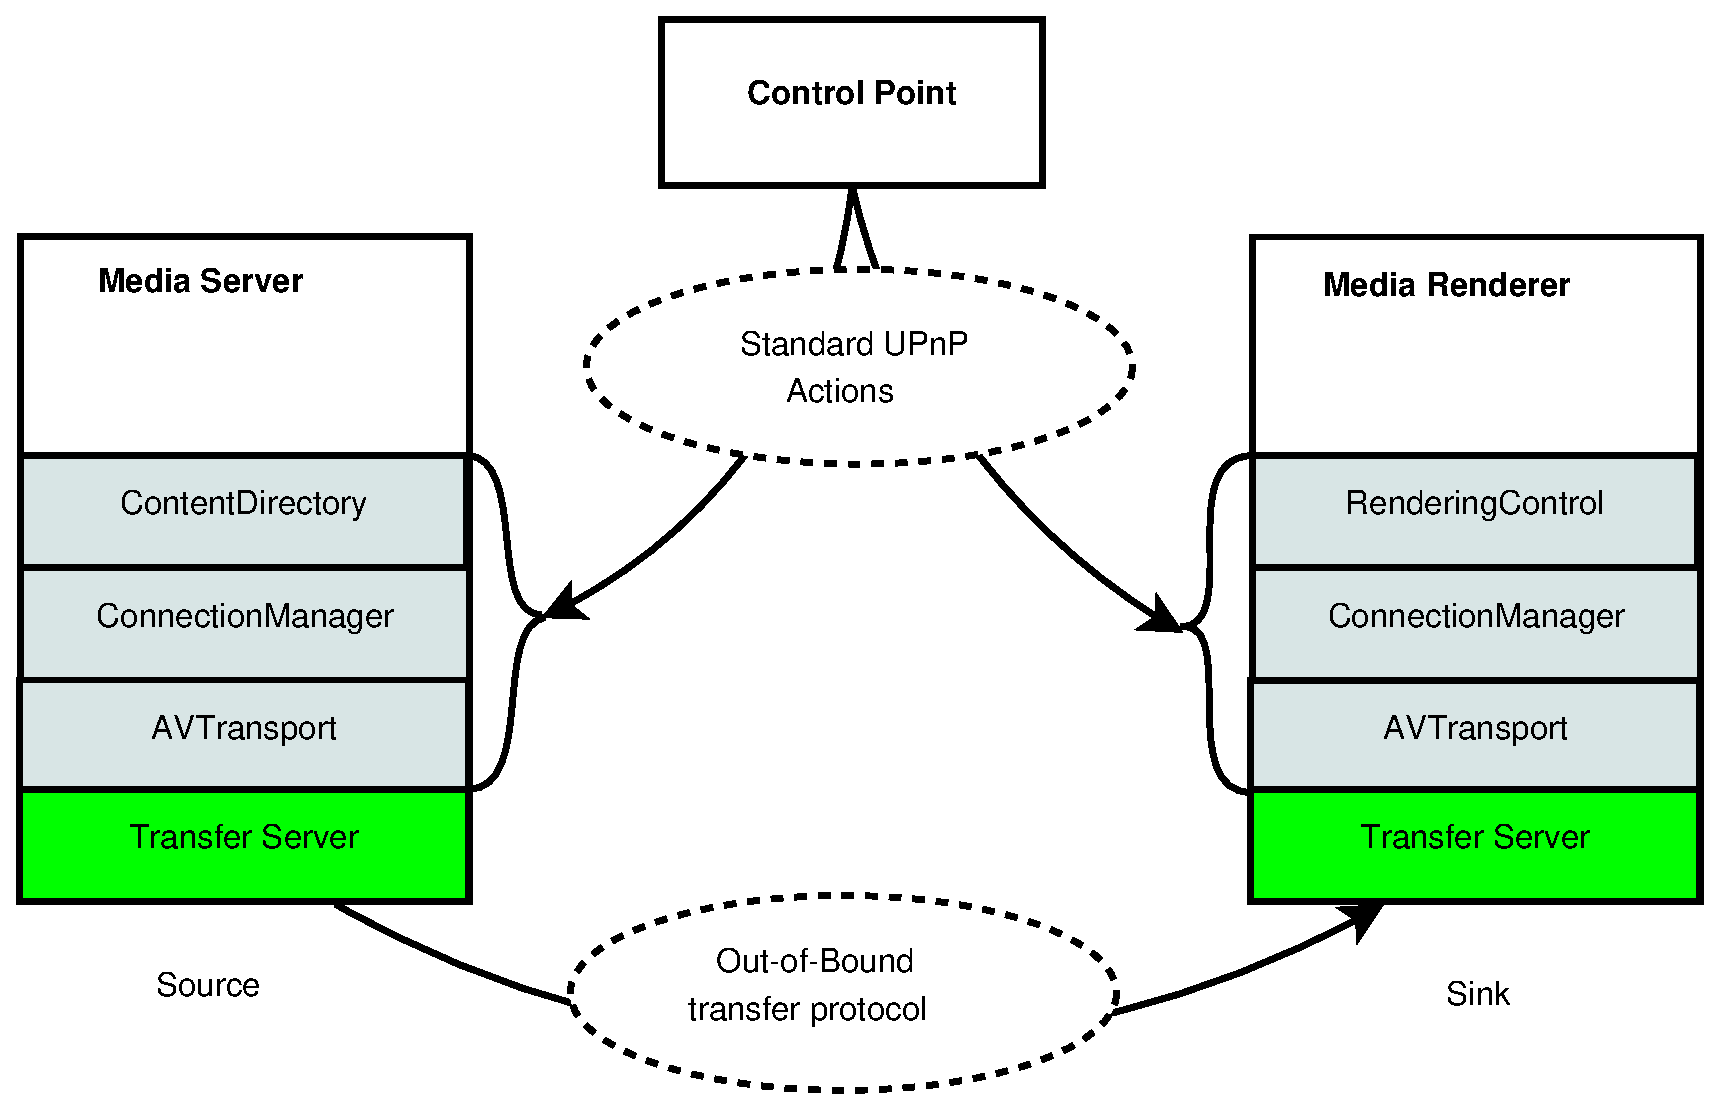
\includegraphics[height=9cm]{charts/upnp_playback} 
\caption{UPnP A/V playback architecture \label{upnp_playback}} 
\end{figure} 

\begin{enumerate} 
\item Media Server \\ 
The media server is used to locate available content in the home network. It's 
primary purpose is to allow control points to enumerate (browse or search) 
content items that are available for the user to render. The media server 
contains a ContentDirectory Service(CDS), a ConnectionManager Service(CM) 
, and an optional AVTransport Service(AVT) which depends on the supported 
transfer protocols. Some media servers are capable of transferring multiple 
content items at the same time. 

The ContentDirectory service is used by the control point to enumerate the content 
on the server. The primary action is ContentDirectroy::Browse(). After 
invoking this action, the control point can obtain detailed information of each 
item that the server can provide. This detailed information includes name, 
artist, date created, size and also the transfer protocols and data formats that 
supported by the for particular item. By parsing this detailed information, 
the control point is able to distinguish whether the item can be rendered by the 
given media renderer. 

The ConnectionManager service is used to manage the connections between a 
control point and a device. The primary action is 
ConnectionManager:: PrepareForConnection(), which is invoked by the control 
point to prepare the server for an upcoming transfer. This 
action will return the instanceID of an AVTransport service that will be used 
later to control, say to stop, pause, seek, the flow of content. The instanceID is used to distinguish multiple instances of the AVTransport service. Since each instance is associated with a particular connection to the renderer, the instanceID enables multiple renderer support at the same time. When the 
control point need to disconnect the connection, it will invoke the media 
server's ConnectionManager::ConnectionComplete() action to release the 
connection. When the ConnectionManager::PrepareForConnection() action is not 
implemented, the control point is only able to support a single renderer at a 
time. In this case 0 will be used as InstanceID. 

The AVTransport service is used by the control point to control the playback of the 
content. Operations like Stop, Pause, Seek are supported by this service. However, this 
service is not mandatory and the media server can choose to implement this feature 
according to the supported transfer protocols and data formats. If this service 
is supported, the InstanceID included in each AVTransport action is used to 
distinguish multiple instances of the service. New instances of the AVTransport 
service can be created by ConnectionManager's 
ConnectionManager::PrepareForConnection() action, and new InstanceID is 
allocated to each new service instance. 

\item Media Renderer \\ 
The media renderer is used to render the content obtained from home 
networking. Its main feature is that it can be discovered by a control point and perform content rendering according to the instructions from the control point. These instructions could control rendering settings such as brightness, contrast, volume, mute, etc. The control of flow of the content like stop, pause, seek can also be supported depending on the transfer protocol used. The media 
renderer provides three services including the RenderingControl service, the ConnectionManager 
service and an optional AVTransport service. Sometimes the rendering control and 
AVTransport services contain multiple independent instances so that the devices 
could be able to handle multiple content items at the same time. Those multiple 
instances can be identified by a unique InstanceID. 

The RenderingControl service is used by the control point to control how the renderer 
renders the incoming content. Characteristics like brightness, contrast, 
volume, mute etc, can be controlled by this service. The RenderingControl service 
supports multiple, dynamic instances, which allows a renderer to mix one or 
more items together. Such a dynamic instance could be a Picture-in-Picture window on a TV or a mixed audio stream. Multiple connections can be distinguished by their unique InstanceID. 

The ConnectionManager service is used to manage connections associated with a 
device, the primary action is the ConnectionManager::GetProtocolInfo() action. 
The control point can invoke this action to enumerate the transfer protocols and 
data formats supported by the media renderer. By comparing this information with 
the protocol information retrieved from the media server, the control point is able to 
predetermine if a media server is capable of rendering a specific item from 
the media server. Optionally, media renderer may also implement the
ConnectionManager::PrepareForConnection() action to prepare itself for an 
upcoming transfer. It can also assign a unique ConnectionID that can be used by 
a 3rd party control point to obtain information about the connections that media 
renderer is using. In addition, depending on the transfer protocol and data 
format used, this action may also return a unique AVTransport InstanceID that the control 
point can use to control the flow of content(stop, pause, seek, etc). 

The AVTransport service is used to control the flow of streamed content. Actions 
like play, stop, pause and seek can be controlled depending on the transfer 
protocol and supported data formats. The AVTransport service can also support 
multiple logical instances and handle multiple simultaneous content items. The 
AVTransport InstanceID which is used to distinguish service instances can be 
allocated by ConnectionManager::PrepareForConnection(). 

\item Control Point \\ 
The Control Point is used to bridge communication between a media server and a media renderer. 
It also provides the user interface to users. A control point does not implement UPnP 
services, as a result it is not visible as a device on the network. Usually the control point 
invokes a media server or a media renderer's services in order to complete the 
desired operations.

The user control point can be used in different scenarios and usually it can 
perform the following functions: 

\begin{itemize} 
\item Discover A/V devices 
\item Locate desired media content 
\item Get renderer's supported protocol and formats 
\item Compare and match protocols and formats between media server and media 
renderer 
\item Configure media server and media renderer 
\item Select desired content 
\item Start content transfer between media server and media renderer 
\item Adjust rendering characteristics 
\item Select next content in the list 
\item Cleanup media server and media renderer 
\end{itemize} 

\end{enumerate} 

As described above, three basic functional entities are defined in the UPnP AV 
architecture\cite{upnp-av}, which are Media Server, Media Renderer and Control Point respectively.
A physical device can consist of a combination of any of these functional 
entities. One typical example is that a DLNA Media player is a combination of a Control 
Point and a Media renderer. 

A simplified UPnP Audio Video 3-box model \cite{DLNA_proxy} can be 
seen as below: 

\begin{figure}[htb] 
\centering 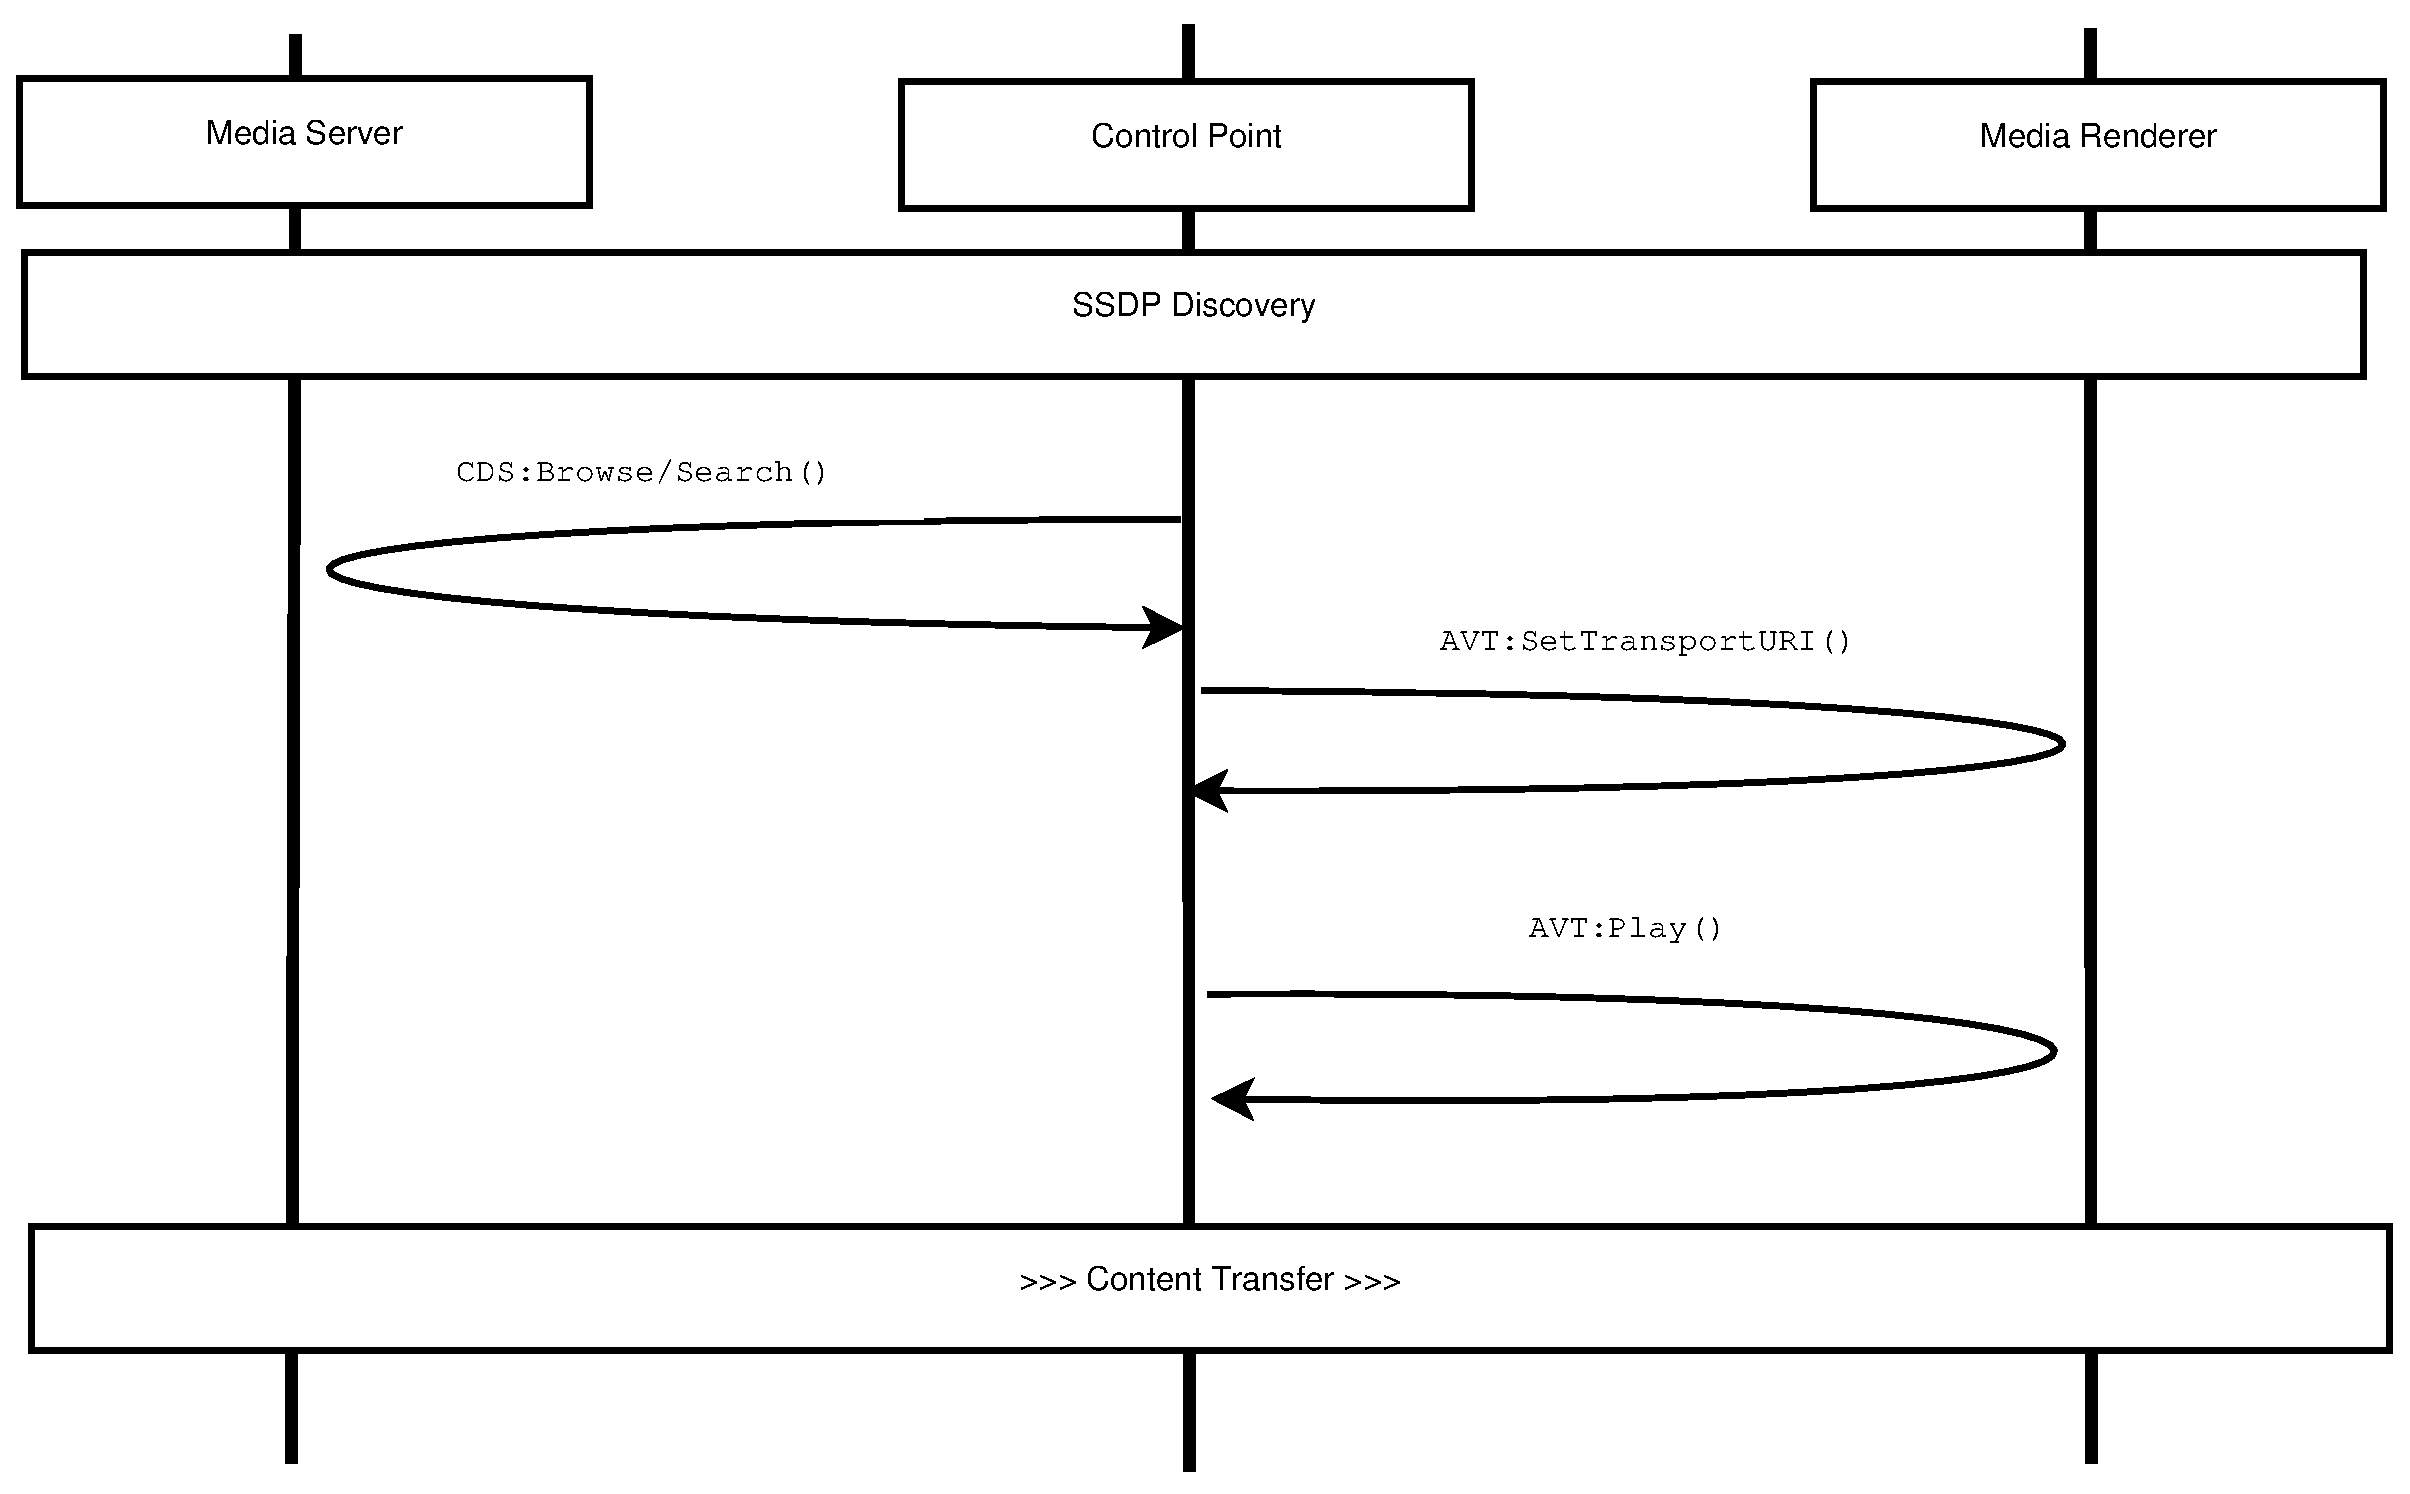
\includegraphics[height=9cm]{charts/chart1} 
\caption{Typical UPnP AV use scenario \label{chart1}} 
\end{figure} 

The first thing in UPnP network communication is the Simple Service Discovery 
Protocol(SSDP)-based device discovery. A SSDP multicast message is sent when a 
new device is added to the network. A control point would listen to these 
multicast messages. On receiving the SSDP message, the control point would send a request for the device's description and services using the location found in the SSDP discovery message. Then the control point can issue the services action command using the Simple Object Access protocol (SOAP). 

In media sharing scenarios, the control point would browse the information about 
the Content Directory Service (CDS) provided by the Media Server. A 
browse/Search action can be invoked to navigate through the content stored in 
the Media Server device. After the control point has selected the media content from 
Media Server, a Media Renderer AVTransport::SetAVTransportURI would be sent by 
the control point to the Media Renderer. Finally, the Play command is invoked by 
the control point to instruct the Media Renderer. Afterward, the transfer begins. The media 
stream travels directly between the Media Server and the Media Renderer, through HTTP, 
RTP or other streaming protocols. 

The media playback control actions can also be invoked by the control point. Methods 
supported include volume control, seek, pause etc. 

\subsubsection[DLNA]{DLNA\footnote{Digital Living Network Alliance}} 
DLNA is a relatively old industry standard compared with other home networking 
solutions. It is mainly based on the UPnP Audio/Video architecture, which is 
discussed in \ref{upnp}. As a result it is widely used by many manufactures. Newer 
home networking solutions are also influenced by DLNA and they follow similar 
technologies used in DLNA. In this paper the DLNA and UPnP standard architectures are studied to help us gain a grasp of how a home networking solution could look like. 

An overview of the DLNA architecture \cite{dlna_guideline} is described below: 
\begin{enumerate} 
\item Architectures and Protocols 

%% table 3, Key Technology Ingredients 
\begin{table}[htb] 
\caption{Key Technology Ingredients \label{Table3}} 
\begin{center} 
\fbox{ 
\begin{tabular}{c|c}  
\textbf { Functional Components } & { Technology Ingredients } \\ \hline 
\textbf Connectivity & Ethernet, 802.11 (including Wi-Fi Direct) \\ 
\textbf  & MoCA, HPNA and Bluetooth \\ \hline 
\textbf Networking & IPv4 Suite \\ \hline 
\textbf Device Discovery and Control & UPnP* Device Architecture v1.0 
\ref{upnpdevice} \\ \hline 
\textbf Media Management and Control & UPnP AV and UPnP Printer:1 
\ref{upnpav}\\ \hline 
\textbf Media Formats & Required and Optional Format Profiles \\ \hline 
\textbf Media Transport & Media Transport \\ \hline 
\textbf Remote User Interfaces & CEA-2014-A 
\end{tabular} 
} 
\end{center} 
\end{table} 

The DLNA architecture is built upon the UPnP protocol, which is discussed in 
 in \ref{upnp}. 
In the network layer DLNA uses the IPv4 suite. On top of the network layer, the UPnP device architecture and UPnP AV architecture is used to control and manage media devices. The DLNA 
guideline also addresses the media format compatibility and media transport 
interoperability issues in support of interoperability among devices. 

\item Media Format Profiles \\ 
DLNA defines the media formats used by the DLNA home networking 
standard. There are three types of media in DLNA: music, video and photo. 
\begin{enumerate} 
\item Music \\ 
Minimal requirement is the LPCM format. Used by PCM raw data, this format is not compressed and it does not require heavy CPU usage. However the bandwidth consumption is 
considerably bigger than other formats. 

MP3 is the most popular music format. It is a compressed format and requires 
some CPU power for encoding or decoding. Compared with LPCM, the bandwidth consumption of MP3 is less, making it suitable for low bandwidth networking. 

AAC is another kind of compressed audio format and it becomes popular since it is the default media format of iTunes. It has similar characteristics of MP3. 
\item Photo \\ 
The minimal requirement in the DLNA guideline is the JPEG format. In many occasions JPEG is the only suggested format due to its proven quality and compress ratio. 
\item Video \\ 
The minimal requirement in DLNA guideline is the MP4 format. The detailed audio and video codecs are also specified in DLNA media format guidelines. 
\end{enumerate} 
In a device-to-device scenario, the media server may store a huge amount of differently 
formatted media. The communication between two devices should follow the same encoding mechanism. Normally the media server takes the responsibility to transcode the media to a certain format defined by the DLNA media format profile guideline. 
\item Link Protection \\ 
DLNA Link Protection is defined as the protection of a content stream between two 
devices on a DLNA network against illegitimate observation or interception. 

Content protection is an important mechanism to ensure that commercial content is protected 
from piracy and illegitimate redistribution. Link Protection is a technique that enables 
distribution of protected commercial content on a home network. It provides protection for copyright holders and content providers without sacrificing consumer flexibility. 
\item Digital rights management (DRM) Interoperability Solutions (DIS) \\ 
DIS is intended to be used to enable the secure transfer and use of protected 
commercial content among different implementations on network media devices. 
The content could be protected by different content protection technologies, 
which are described as DRMs in short. 
\item Device Profiles \\ 
A Device Profile is a collection of DLNA capabilities and features within a DLNA device. For a device 
to be compliant with a Device Profile, it has to conform to all of the guidelines listed for that 
Device Profile. 

In practice, Device Profiles reference existing optional or recommended DLNA guidelines that enable certain features, and makes those DLNA guidelines mandatory within the context of a Device Profile. 
A Device Profile can also provide some additional guidelines that complement or modify existing DLNA guidelines for a feature. 

A particular type of DLNA Device Profile is the Commercial Video Profile (CVP). A CVP Device Profile is an extension of the DLNA guidelines that will allow content from service providers and multichannel video programming distributers to be distributed on the DLNA network. DLNA Commercial Video Profiles (CVPs) are defined as Device Profiles that consistently enable commercial content that enters the home network through a gateway device via an interface to a commercial content service provider. Since different regions of the world have different requirements for commercial content, there are multiple CVPs defined. 

\end{enumerate} 

\subsubsection{AirPlay} 
AirPlay is Apple Inc's home networking solution. It is a family of protocols 
used to display different types of media content on Apple TV from other iOS devices. 
AirPlay support multiple functions, including displaying photos and sideshows from iOS devices, streaming audio from iOS devices or iTunes, as well as displaying videos from iOS device and 
showing the whole screen on Apple TV, which is known as AirPlay Mirroring. 

AirPlay's specification is not open to public. However unofficial specifications have been made by some hackers through reverse engineering the protocol stack \cite{AirPlay-spec}. These unofficial specifications could be found on the Internet \cite{AirPlay-spec}.  
The specification includes 6 parts, which are described below: 

\begin{enumerate} 
\item Service Discovery \\ 
The service discovery of AirPlay stems from the IETF Zeroconf Working Group, 
who is dedicated to improve the ease-of-use (Zero Configuration) of networks. The 
Zeroconf working group has made it possible to make two devices in the 
network to communicate effectively using IP, without requiring a specialist to manually 
configure the network. 

AirPlay's service discovery is based on Multicast DNS \cite{multicastdns}, which 
fulfills the Zeroconf requirement. Multicast DNS is a way of using familiar DNS 
programming interfaces, packet formats and operating semantics, in a small 
network where no conventional DNS server has been installed. The requirements 
for Zeroconf name resolution could be met by designing an entirely new 
protocol, since it is better to provide this functionality by making minimal changes 
to the current standard DNS protocol. By using Multicast DNS, most current 
applications need no changes at all to work correctly using mDNS in a Zeroconf network. Besides,
engineers do not have to learn an entirely new protocol. Moreover current network 
packet capture tools are already capable of  decoding and displaying the DNS packets. Thus they do not 
have to be updated to understand new packet formats. 

An AirPlay device such as the Apple TV publishes two services. The first one is 
RAOP (Remote Audio Output Protocol), used for audio streaming. The second 
one is the AirPlay service, used for photos and video content. 

The AirPlay server is an HTTP server (RFC 2616). Two connections are made to this 
server, with the second one being used as a reverse HTTP connection. This allows a 
client to receive asynchronous events, such as playback status changes, from a 
server. 
\item Video streaming \\ 
The video streaming uses typical HTTP streaming technology, the controller set 
the streaming URL to Apple TV or other AirPlay receiver. While the URL is set, 
Apple TV start to download video from the server using the URL and starts 
playing while buffered enough data. The control messages can be seen in 
table \ref{video_stream}. 

Note that the Apple TV does not support Video Volume Control. 
%% table , Video Streaming 
\begin{table}[htb] 
\caption{AirPlay Video Control HTTP requests \label{video_stream}} 
\begin{center} 
\fbox{ 
\begin{tabular}{c|l|l}  
\textbf { Method } & { Request } & { Description }\\ \hline 
\textbf GET & /server-info & Fetch general informations about the AirPlay server \\ \hline 
\textbf POST & /play & Start video playback \\ \hline 
\textbf POST & /scrub & Seek at an arbitrary location in the video \\ \hline 
\textbf POST & /rate & Change the playback rate,0 is paused, 1 is normal \\ 
\hline 
\textbf POST & /stop & Stop playback \\ \hline 
\textbf GET & /scrub & Retrieve the current playback position \\ \hline 
\textbf GET & /playback-info & Retrieve playback informations like position, 
duration\ldots \\ \hline 
\textbf PUT & /setProperty & Set playback property \\ \hline 
\textbf GET & /getProperty & Get playback property 
\end{tabular} 
} 
\end{center} 
\end{table} 
\item Photo streaming \\ 
The image streaming uses HTTP put message to send image raw data to Apple TV or 
other devices, when the whole image is received, the image is then rendered on 
screen. The AirPlay also supports slide show, the control message can be seen in 
table \ref{photo_stream}. 
\begin{table}[htb] 
\caption{AirPlay Photo Control HTTP requests \label{photo_stream}} 
\begin{center} 
\fbox{ 
\begin{tabular}{c|l|l}  
\textbf { Method } & { Request } & { Description }\\ \hline 
\textbf GET & /slideshow-features & Fetch the list of available transitions for slideshows \\ \hline 
\textbf PUT & /photo & Send a JPEG picture to the server \\ \hline 
\textbf PUT & /slideshows/1 & Start or stop a slideshow session \\ 
\hline 
\textbf POST & /stop & Stop a photo or slideshow session 
\end{tabular} 
} 
\end{center} 
\end{table} 
\item Music streaming \\ 
AirPlay music streaming is a bit different from video and image streaming, the 
technology used is RTSP streaming, it is more "push like" protocol, the RTSP 
streaming server push UDP packets to receiver. However the RTSP protocol Apple 
used is not standard RTSP, it uses its own implementation, called  RAOP (Remote 
Audio Output Protocol). The control message can be seen in table 
\ref{music_stream}. 
\begin{table}[htb] 
\caption{AirPlay Audio Control RTSP requests \label{music_stream}} 
\begin{center} 
\fbox{ 
\begin{tabular}{c|l}  
\textbf { RTSP request } & { Description }\\ \hline 
\textbf OPTIONS & Ask the RTSP server for its supported methods \\ \hline 
\textbf ANNOUNCE & Tell the RTSP server about stream properties using SDP \\ 
\hline 
\textbf SETUP & Initialize a record session \\ \hline 
\textbf RECORD & Start the audio streaming \\ \hline 
\textbf FLUSH & Stop the streaming \\ \hline 
\textbf TEARDOWN & End the RTSP session 
\end{tabular} 
} 
\end{center} 
\end{table} 

\item Screen mirroring \\ 
AirPlay screen mirroring is achieved by transmitting H.264 encoded video stream 
over a TCP connection. The stream is packetized with a 128-byte header. The 
audio is sent using AirTunes protocol and AAC-ELD formatted. 
NTP(Network time protocol) is used for synchronization. The synchronization 
takes place on UDP port 7010(client) and 7011(server), using NTP protocol. The 
AirPlay server runs a NTP client. Request are sent to AirPlay client at 3 
second intervals. The reference date for time stamp is the beginning of the 
mirroring session.  The control message can be seen in table 
\ref{mirroring_stream}. 
\begin{table}[htb] 
\caption{AirPlay Mirroring Control HTTP requests \label{mirroring_stream}} 
\begin{center} 
\fbox{ 
\begin{tabular}{c|l|l}  
\textbf { Method } & { Request } & { Description }\\ \hline 
\textbf GET & /stream.xml & Retrieve information about the server capabilities 
\\ \hline 
\textbf POST & /stream & Start the live video transmission 
\end{tabular} 
} 
\end{center} 
\end{table} 
\item Authentication \\ 
An AirPlay server can require a password for displaying any content from the 
network. It is implemented using standard HTTP Digest Authentication (RFC 2617), 
over RTSP for AirTunes, and HTTP for everything else. Te digest realms and 
usernames accepted by Apple TV are described in table \ref{hda}. 
%% table , AirPlay Authentication 
\begin{table}[htb] 
\caption{AirPlay HTTP Digest Authentication \label{hda}} 
\begin{center} 
\fbox{ 
\begin{tabular}{c|c|c}  
\textbf { Service } & { Realm } & { Username }\\ \hline 
\textbf AirTunes & roap & iTunes \\ \hline 
\textbf AirPlay & AirPlay & AirPlay 
\end{tabular} 
} 
\end{center} 
\end{table} 
\end{enumerate} 

\subsubsection{DIAL} 
Chromecast and FireTV use the DIAL \cite{dial} (DIscovery And Launch) protocol, 
co-developed by Netflix and YouTube, to search for available devices on a Wi-Fi network. 
Once a device is discovered, the protocol synchronizes information on how to 
connect to the device. The protocol is proposed by Google and Netflix so the 
YouTube and Netflix application has already build in with DIAL device discovery. The 
streaming part uses HTTP streaming, which means controller can directly set the 
streaming URL and the receiver will start downloading automatically. 

The DIAL protocol has two components: DIAL Service Discovery and the DIAL 
Representational State Transfer (REST) Service. DIAL Service Discovery enables a 
DIAL client device to discover DIAL servers on its local network segment and 
obtain access to the DIAL REST Service on those devices. The DIAL REST Service 
enables a DIAL client to query, launch, and optionally stop applications on a 
DIAL server device. 
\begin{enumerate} 
\item DIAL Service Discovery \\ 
The DIAL Service Discovery protocol is based on Simple Service Discovery 
Protocol (SSDP), which is defined as part of UPnP device architecture discussed 
in \ref{upnp}. 

A DIAL client will firstly send an M-Search request over UDP to the IPv4 
multicast address 239.255.255.250 and UDP port 1900 including the Search Target 
header. After that the SSDP/UPnP server responds including a LOCATION header 
containing an absolute HTTP URL for the UPnP description of the root device. 
When receives the M-SEARCH response, the DIAL client will send an HTTP GET 
request to the URL received in the LOCATION header of the M-SEARCH response to 
get HTTP response containing the UPnP device description as a XML content. The 
overall flow of DIAL discovery is shown in figure \ref{dial_discovery}. 

\begin{figure}[htb] \centering 
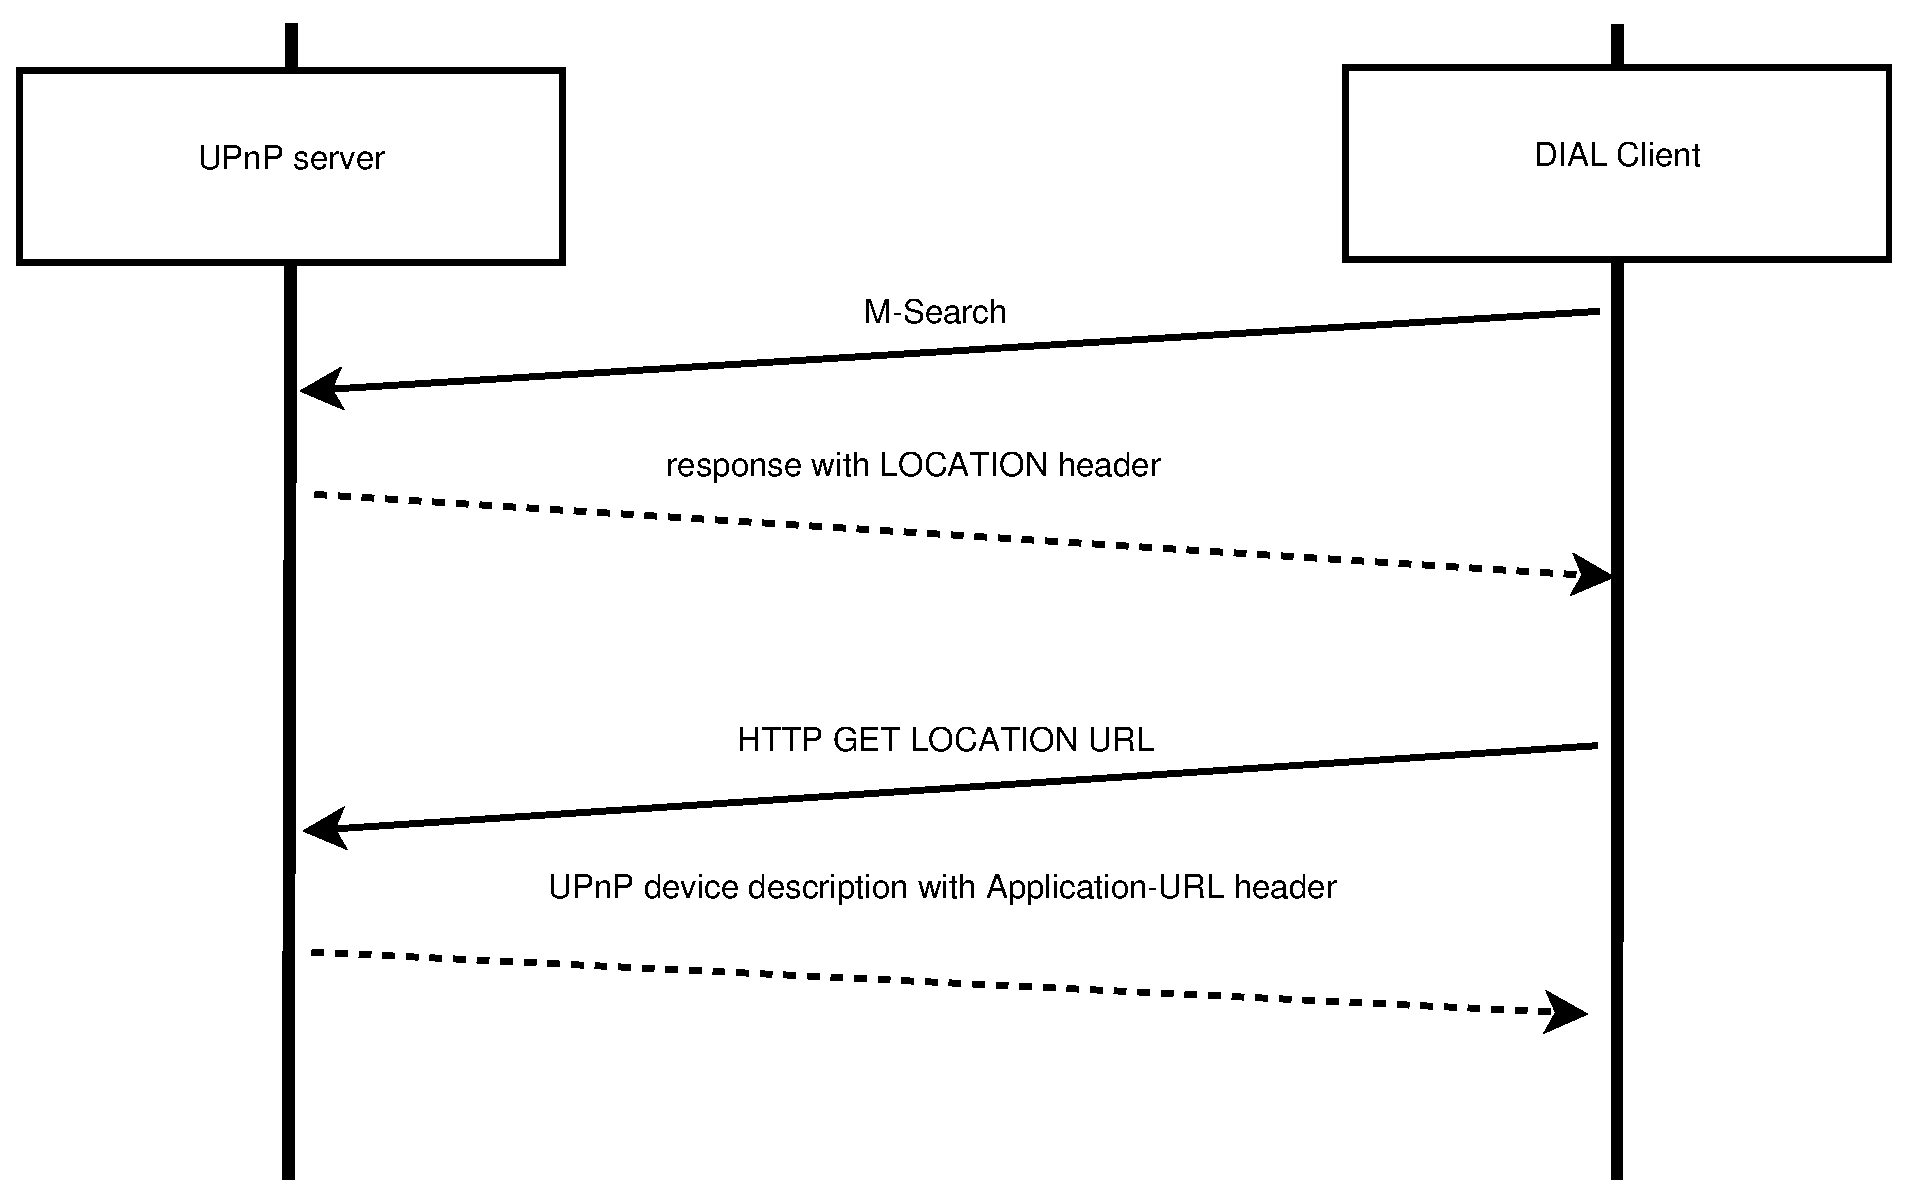
\includegraphics[height=9cm]{charts/dial_discovery} 
\caption{DIAL Discovery \label{dial_discovery}} 
\end{figure} 

\item DIAL REST Service \\ 
The DIAL REST service allocates URLs for different resource applications such as 
YouTube and Netflix. Then the application can be controlled by issuing HTTP 
requests against the URL for that application. The Application resource URL is 
constructed by concatenating the DIAL REST service URL, a single slash charater 
('/') and the application name. The application name must be registered in DIAL 
Registry to be used. 

A DIAL client firstly send a HTTP GET request to the application resource URL, 
then the server will extract the application name and search for the 
application is installed or not, if the application is not recognized, the 
server will return 404 Not Found or trigger the installation of the specific 
application that is not currently installed, otherwise, the DIAL server return 
an HTTP response with 200 OK and a body contains MIME type in XML. 

The client then sends a HTTP POST request to the application resource URL to 
launch the desired application. On receipt of a valid POST request, the DIAL 
server will extract the application name and run the application, and then send 
a HTTP response with LOCATION header to inform the absolute HTTP URL which 
identifies the running instance of the application. 

The first-screen application can also send small amount of data to the DIAL 
server, and then DIAL server can communicate the information to DIAL clients. 
After the application is launched and communication is established, the DIAL 
client can communicate directly with the application. DIAL REST service overall 
flow chart can be shown as figure \ref{dial_rest}. 

\begin{figure}[htb] \centering 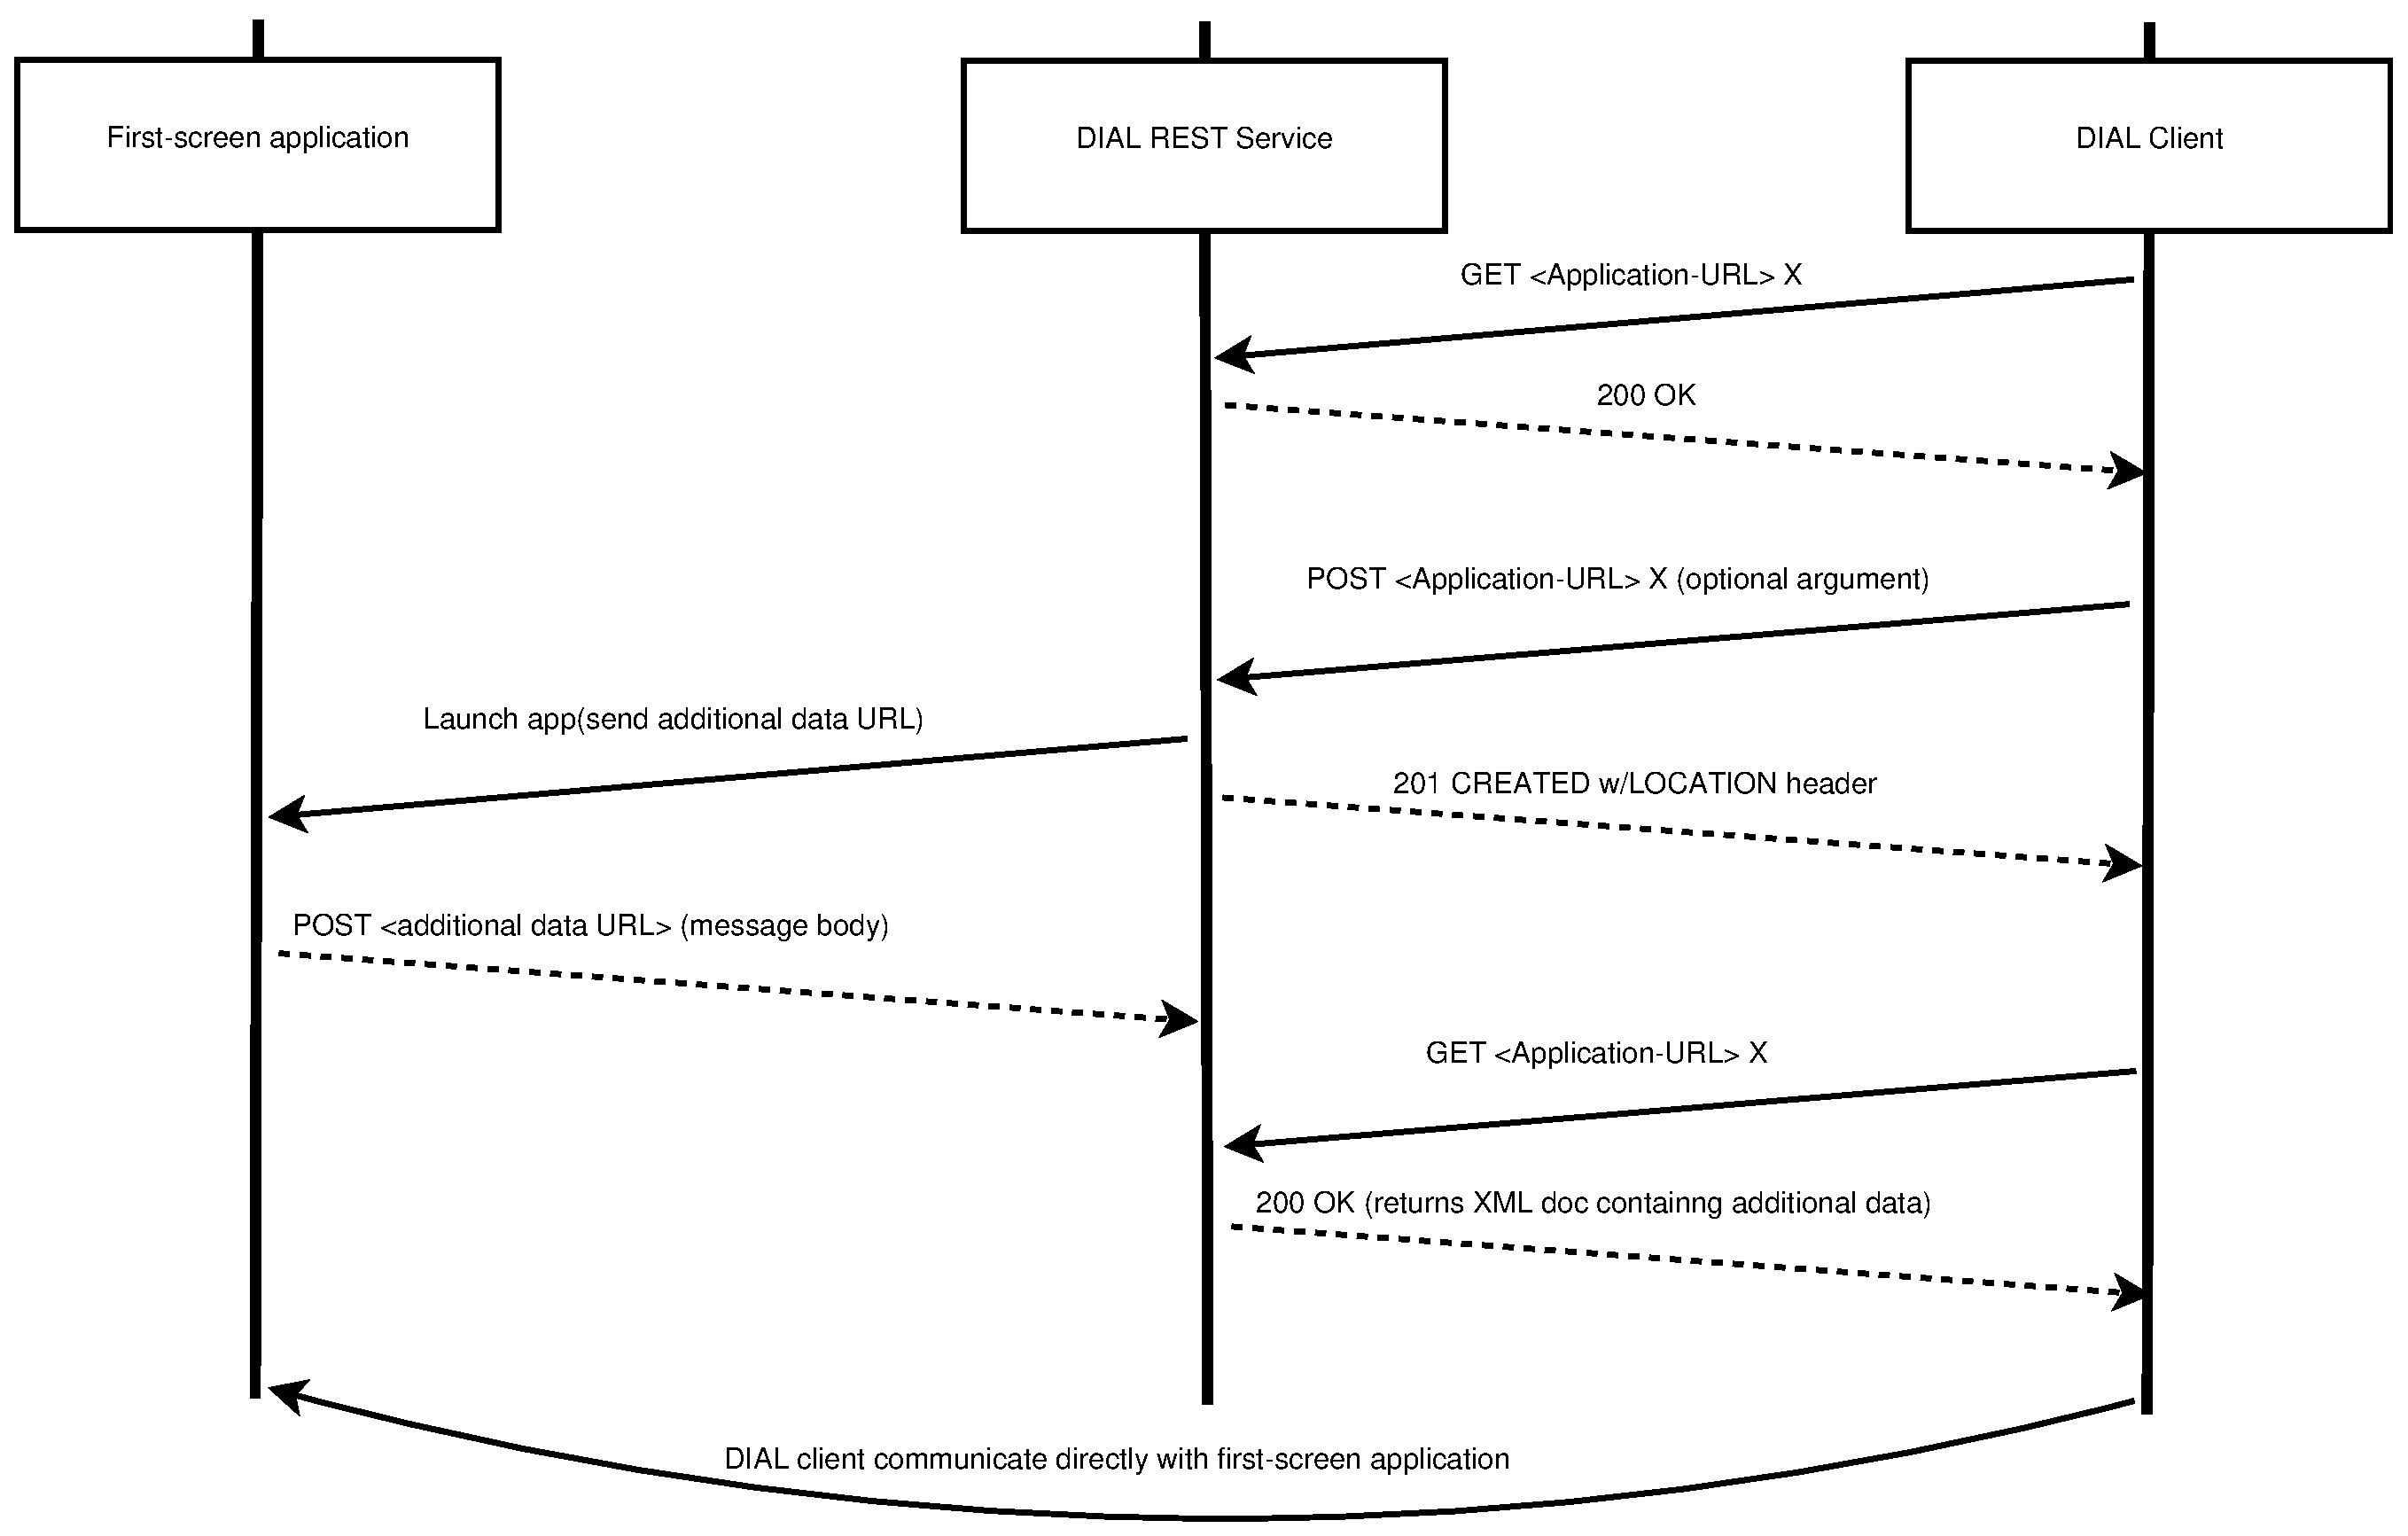
\includegraphics[height=9cm]{charts/dial_rest} 
\caption{DIAL REST service: application launch \label{dial_rest}} 
\end{figure} 
\end{enumerate} 

\subsubsection{Miracast} 

Miracast \cite{miracast_industry} is quit different on technology perspective, 
instead of connecting on the same local network segment, a Wi-Fi peer to peer 
connection is created, so Miracast is not limited to pre-configured network infrastructure. 

Miracast allows users to establish a direct Wi-Fi connection between two 
devices, eliminating the need for an existing network. 

Miracast uses many of the building blocks that, over the years, have enriched 
the user experience and increased their trust in Wi-Fi, including Wi-Fi 
CERTIFIED n (improved throughput and coverage), Wi-Fi Direct (device-to- 
device connectivity), Wi-Fi Protected Access 2 (WPA2) (security), Wi-Fi 
Multimedia (WMM) (traffic management) and Wi-Fi Protected Setup. Some 
Miracast devices will also support Tunneled Direct Link Setup (TDLS), which 
allows them to connect via an infrastructure network. TDLS enables more 
efficient data transfer and the use of more advanced Wi-Fi capabilities than 
those supported by the legacy infrastructure network through which the devices 
are connected. 

Miracast does not require a typical Wi-Fi infrastructure network, though many 
devices will take advantage of network connectivity to access content. Miracast 
connections are expected to be predominantly established between Wi-Fi devices 
connected with each other directly, without an AP acting as an intermediary. 
The direct link between devices is established either through Wi-Fi direct, a 
feature that all Miracast devices are required to support, or through TDLS, an 
option feature. When two devices connect with each other directly, one fulfills 
its role as the source(the transmitting device) and the other functions as a 
display(the device receiving and rendering the content to the user). Topologies 
supported by Miracast are shown in Figure \ref{miracast_model}. 

\begin{figure}[htb] \centering 
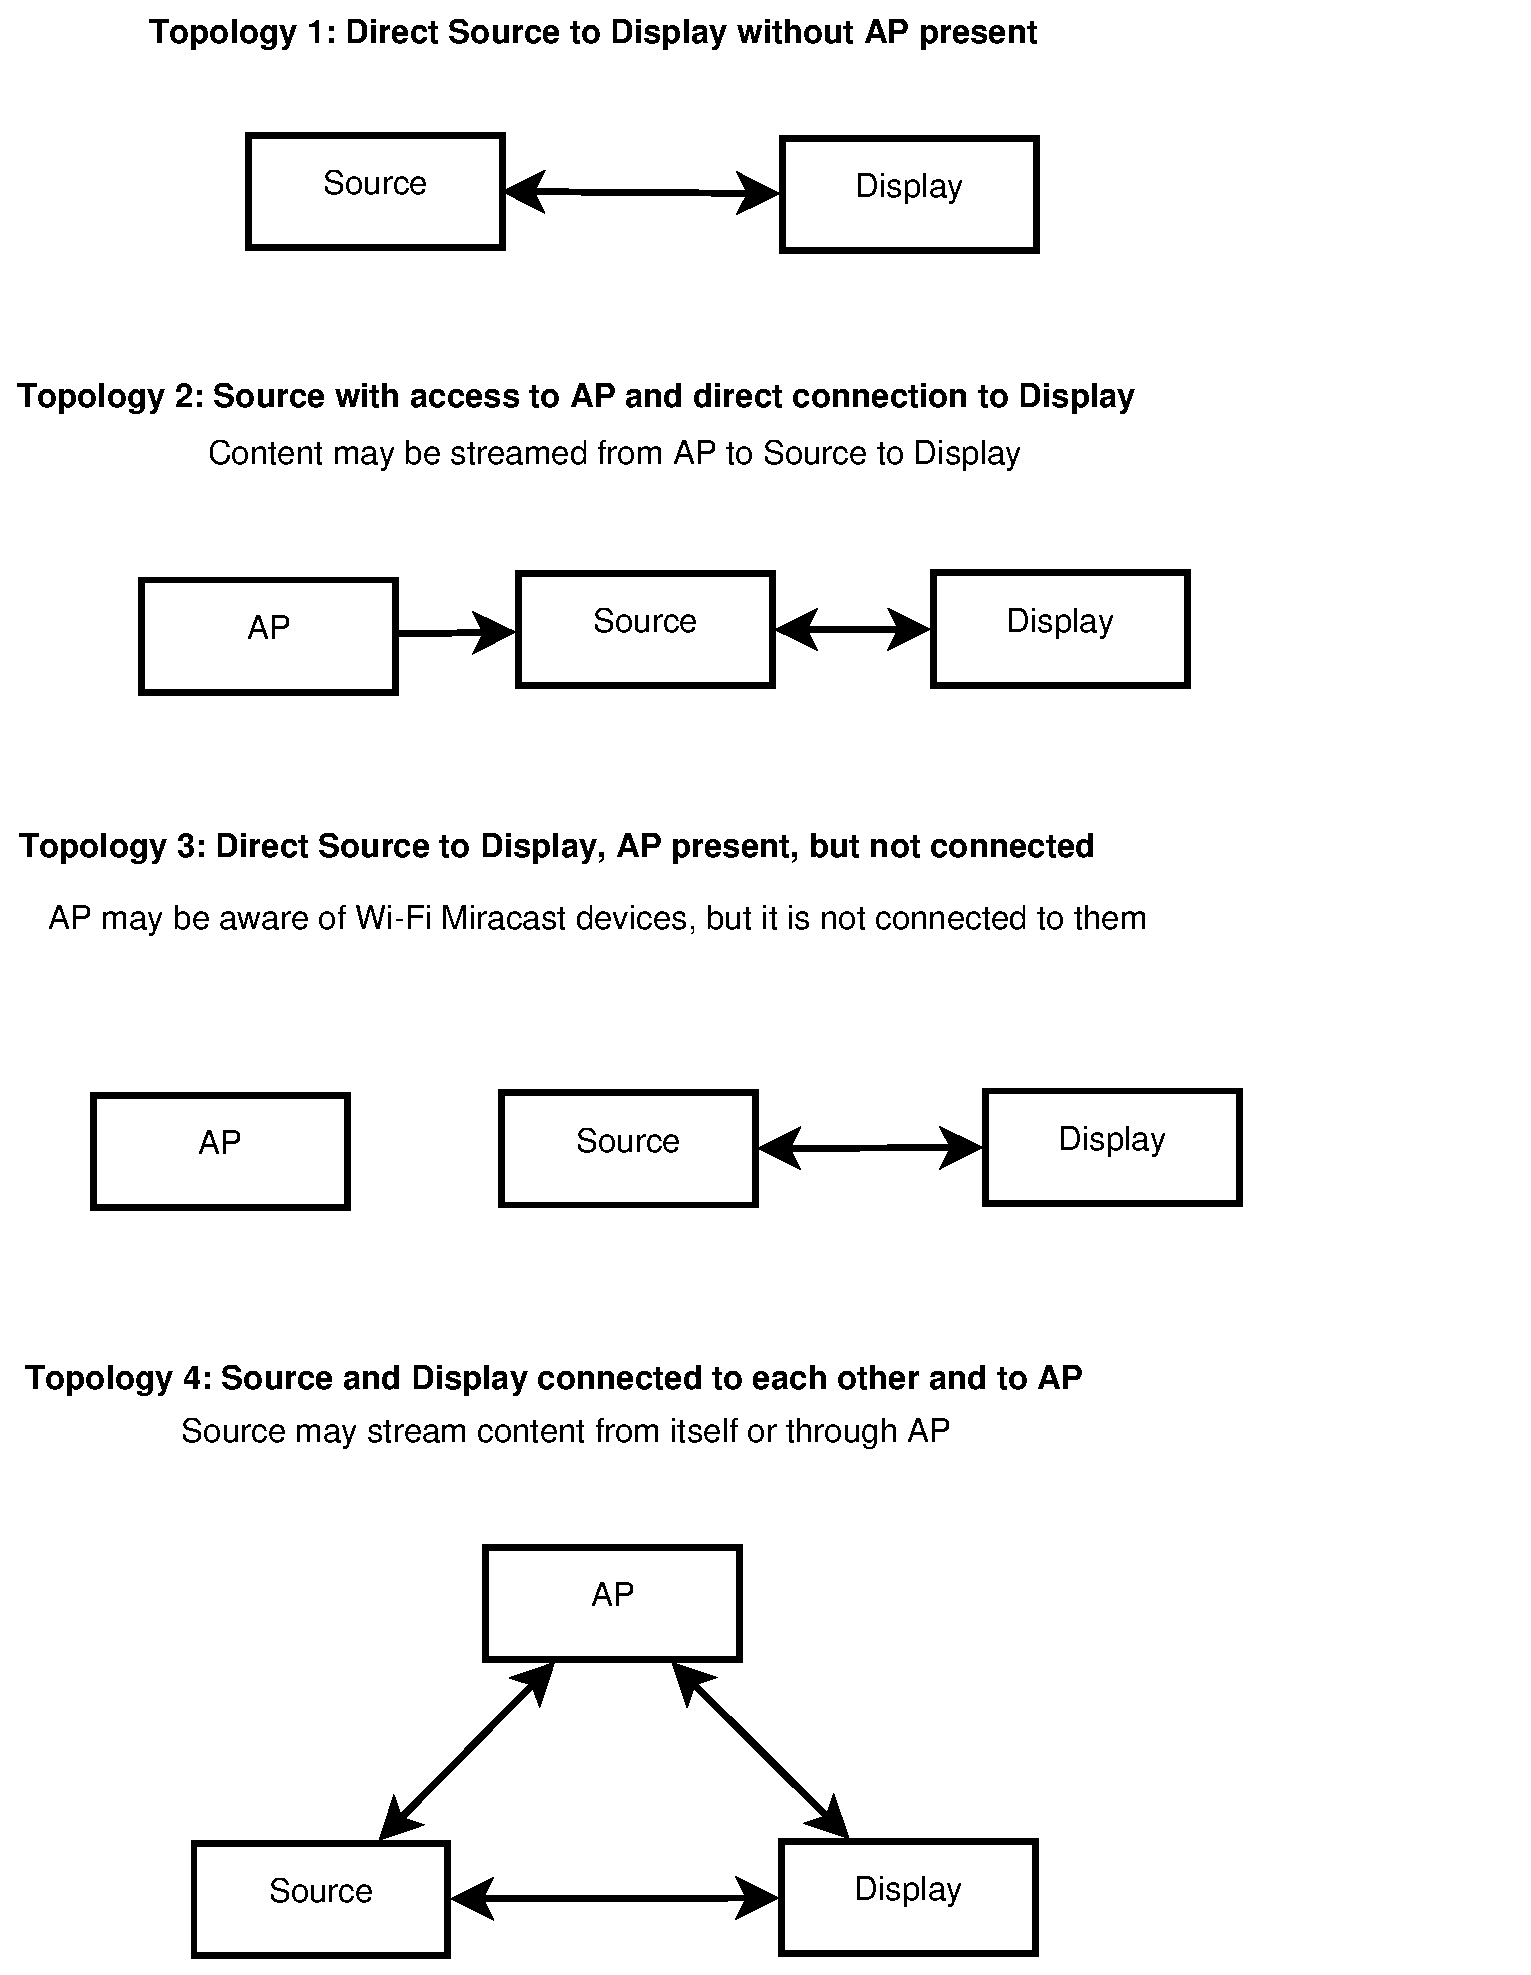
\includegraphics[height=14cm]{charts/miracast_model} 
\caption{Miracast topologies \label{miracast_model}} 
\end{figure} 

On technology perspective, Miracast is built upon many diffenet Wi-Fi 
technologies, which is shown in figure \ref{miracast_architect}. 

\begin{figure}[htb] \centering 
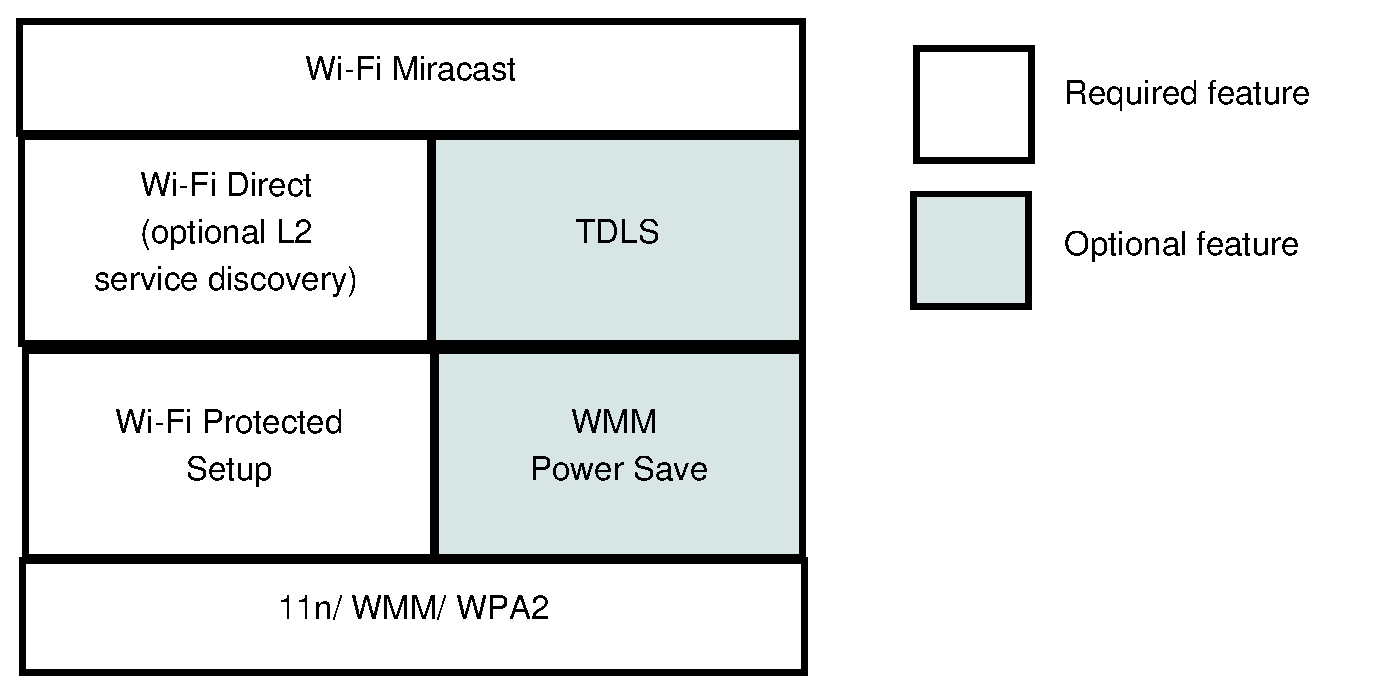
\includegraphics[height=5cm]{charts/miracast_technology_architecture} 
\caption{Miracast technology architecture \label{miracast_architect}} 
\end{figure} 

The technology component includes the following: 
\begin{enumerate} 
\item Connectivity\\ 
Wi-Fi CERTIFIED n provides a transmission channel designed to support 
multimedia content. 
\item Device-to-device connectivity\\ 
Wi-Fi Direct allows devices to connect directly to each other, without the 
need for a Wi-Fi AP, and often requiring just the push of a button. TDLS allows 
devices that are associated to the same Wi-Fi network to establish a direct 
link with each other. 
\item Security\\ 
WPA2 makes the transport of multimedia content safe, 
protecting both the source and the display. 
\item Quality of service (QoS)\\ 
Wi-Fi Multimedia (WMM) gives real-time content, such as voice and audio, 
priority where appropriate over best-effort traffic, to support a good user 
experience. 
\item Battery life \\ 
WMM Power Save extends the battery life of mobile devices 
like smartphones or tablets by minimizing the time the device is actively 
connected to the AP during idle time. Power save mechanisms in Wi-Fi Direct 
provide similar benefits when connecting devices without an AP. 
\item Ease of installation\\ 
Wi-Fi Protected Setup helps users to automatically configure Wi-Fi networks, 
enable WPA2 security, and add new devices. 
\end{enumerate} 

Miracast Session management 

\begin{center} 
    \begin{tabular}{ | p{3.5cm} | p{10cm} |} 
     \hline 
    \multicolumn{2}{c}{Miracast Session Management}\\ 
    \hline 
    Device Discovery  & Source and display devices discover each other prior to 
    connection setup. The Device discovery mechanism is defined in the Wi-Fi 
    Peer-to-Peer (P2P) Specification. \\ \hline 
    
    Service Discovery  & Source and display devices discover each other's 
    Miracast capabilities prior to connection setup. The Service discovery 
    mechanism is defined in the Wi-Fi P2P specification. \\ \hline 
    
    Device selection &A remote device is selected for connection setup. User 
    input and local policies may be used to decide which device is a display 
    and which is a source. \\ \hline 
    
    Connection setup & Connection setup selects a method (Wi-Fi Direct or TDLS) 
    to manage the connection. Wi-Fi Direct sets up a group owner and client to 
    initiate a device-to-device link. A WPA2 single-hop link with selected 
    devices is established. Upon the establishment of connectivity between the 
    source and display devices, the display initiates a Transmission Control 
    Protocol (TCP) connection, with a control port using Real-Time Streaming 
    Protocol (RTSP) to create and manage the sessions between source and 
    display devices. \\ 
    \hline 
    
    Capability negotiation & Source and display devices determine the parameters 
    for the Miracast session. \\ \hline 
    
    Content protection setup (optional) & If the devices support content 
    protection and are streaming content requiring protection, session keys for 
    link content protection are derived using High-bandwidth Digital Content 
    Protection (HDCP) 2.0/2.1. HDCP session keys are established before the RTP 
    session is initiated. This feature is designed to protect the digital 
    rights of content owners and to encourage their efforts to make their 
    content available. \\ \hline 
    
    Session establishment and streaming & Upon completion of capability 
    negotiation, the source and display devices setup the Miracast session 
    prior to streaming content. 
    The audio and video content available on the source device is packetized 
    using Moving Picture Experts Group 2 Transport Stream (MPEG2-TS) coding and 
    encapsulated by Real-Time Protocol (RTP) User Datagram Protocol (UDP) and 
    Internet Protocol (IP). Finally, IEEE 802.11 packetization enables the 
    source device to send content to the display device. \\ \hline 
    
    User input back channel setup (optional) & A User Interface Back Channel 
    (UIBC) for transmitting control and data information related to user 
    interaction with the user interface is set up. User inputs at a display are 
    packetized using a UIBC packet header and transported using Transmission 
    Control Protocol/Internet Protocol (TCP/IP).\\ \hline 
    \end{tabular} 
\end{center} 

\begin{center} 
    \begin{tabular}{ | p{3.5cm} | p{10cm} |} 
     \hline 
    \multicolumn{2}{c}{Miracast Session Management}\\ 
    \hline 
    Payload control & When the payload transfer starts, devices may adapt 
    transmission parameters on the basis of channel conditions and power 
    consumption. Adaptation can be achieved by: Compression ratio change and 
    macroblock skipping (using the H.264 standard); Frame skipping (if the 
    display device supports this functionality, the source device may skip some 
    of the frames to be transmitted according to the current resolution); 
    Format change. \\ \hline 
    
    Display session teardown  & Either the source or the display terminates the 
    Miracast session. \\ \hline 
    \end{tabular} 
\end{center} 

\subsubsection{Other protocols} 
Apart from all mentioned standards above, many other companies or associations 
also proposed their own protocols, for example SonosNet \cite{sonosnet} which is 
based on peer to peer network, and Spotify Connect \cite{spotifyconnect}. The 
standard war on home networking has never end. 

\subsection{Comparison of existing solutions} 
\subsubsection{History} 
\begin{itemize} 
\item[--]DLNA is proposed by several leading consumer electronic manufactures based on UPnP 
technology, from early 2000s on, over 2.2 billion devices has shipped with DLNA solutions, 
making it possible to sharing audio and video seamlessly different smart devices. DLNA alliance 
had two annually meetings a year to discuss the marketing and developing related issues, making 
it a more and more accomplished standard. 

\item[--]AirPlay, on the other hand, is proposed by Apple Inc. in 2010, before that actually 
Apple is a part of DLNA alliance, by proposing AirPlay, it enables more advanced features than 
DLNA, such as whole screen mirroring, RTP audio streaming, authentication etc. 
\item[--]Miracast is a quite new technology, it is formerly known as Wi-Fi Display, and proposed 
in 2012 by Wi-Fi alliance. Different from AirPlay and DLNA, it is not based on home AP, but  
Wi-Fi direct instead. It provides a screen-mirroring feature just like Apple AirPlay Mirroring, 
and now it becomes quite popular among manufactures and software ventures. Google has launched 
its Android 4.2 with native support of Miracast, the latest Kitkat Android 4.4 has been certified 
to the Wi-Fi Alliance Wi-Fi Display Specification as Miracast compatible. There is a strong trend 
that this standard will soon be very popular in multi-screen sharing market. 
\item[--]Chromecast or Google cast is another new trend in 
market, Released in 2013, a piece of 2.83-inch (72 mm) dongle hardware is 
becoming a hot topic recently, with 35\$ price, it has been ranked as the most 
popular device in its category. The standard is proposed by joint effort form 
Google and Netflix, and as they are Internet companies, the standard is 
actually based on Cloud, the content is directly streamed from YouTube and 
Netflix to the Chromecast dongle. And applications running on mobile platforms 
are just acting as a control point. It also provides features like browser 
mirroring, with a Chromecast plugin, a Chrome browser can stream its tab to the 
big screen TV. In a foreseeable future, the standard could become more and more popular. 
\end{itemize} 
\subsubsection{Market} 
\begin{itemize} 
\item[--]DLNA is one of the first proposed solutions for multimedia home 
networking, thus it is so far the most accepted solution, figure 
\ref{dlna_market} shows the growth of DLNA-certified device sales. In 2018, the 
sales will reach 7.32 billion, nearly the totally population of earth. 

\begin{figure}[htb] 
\centering 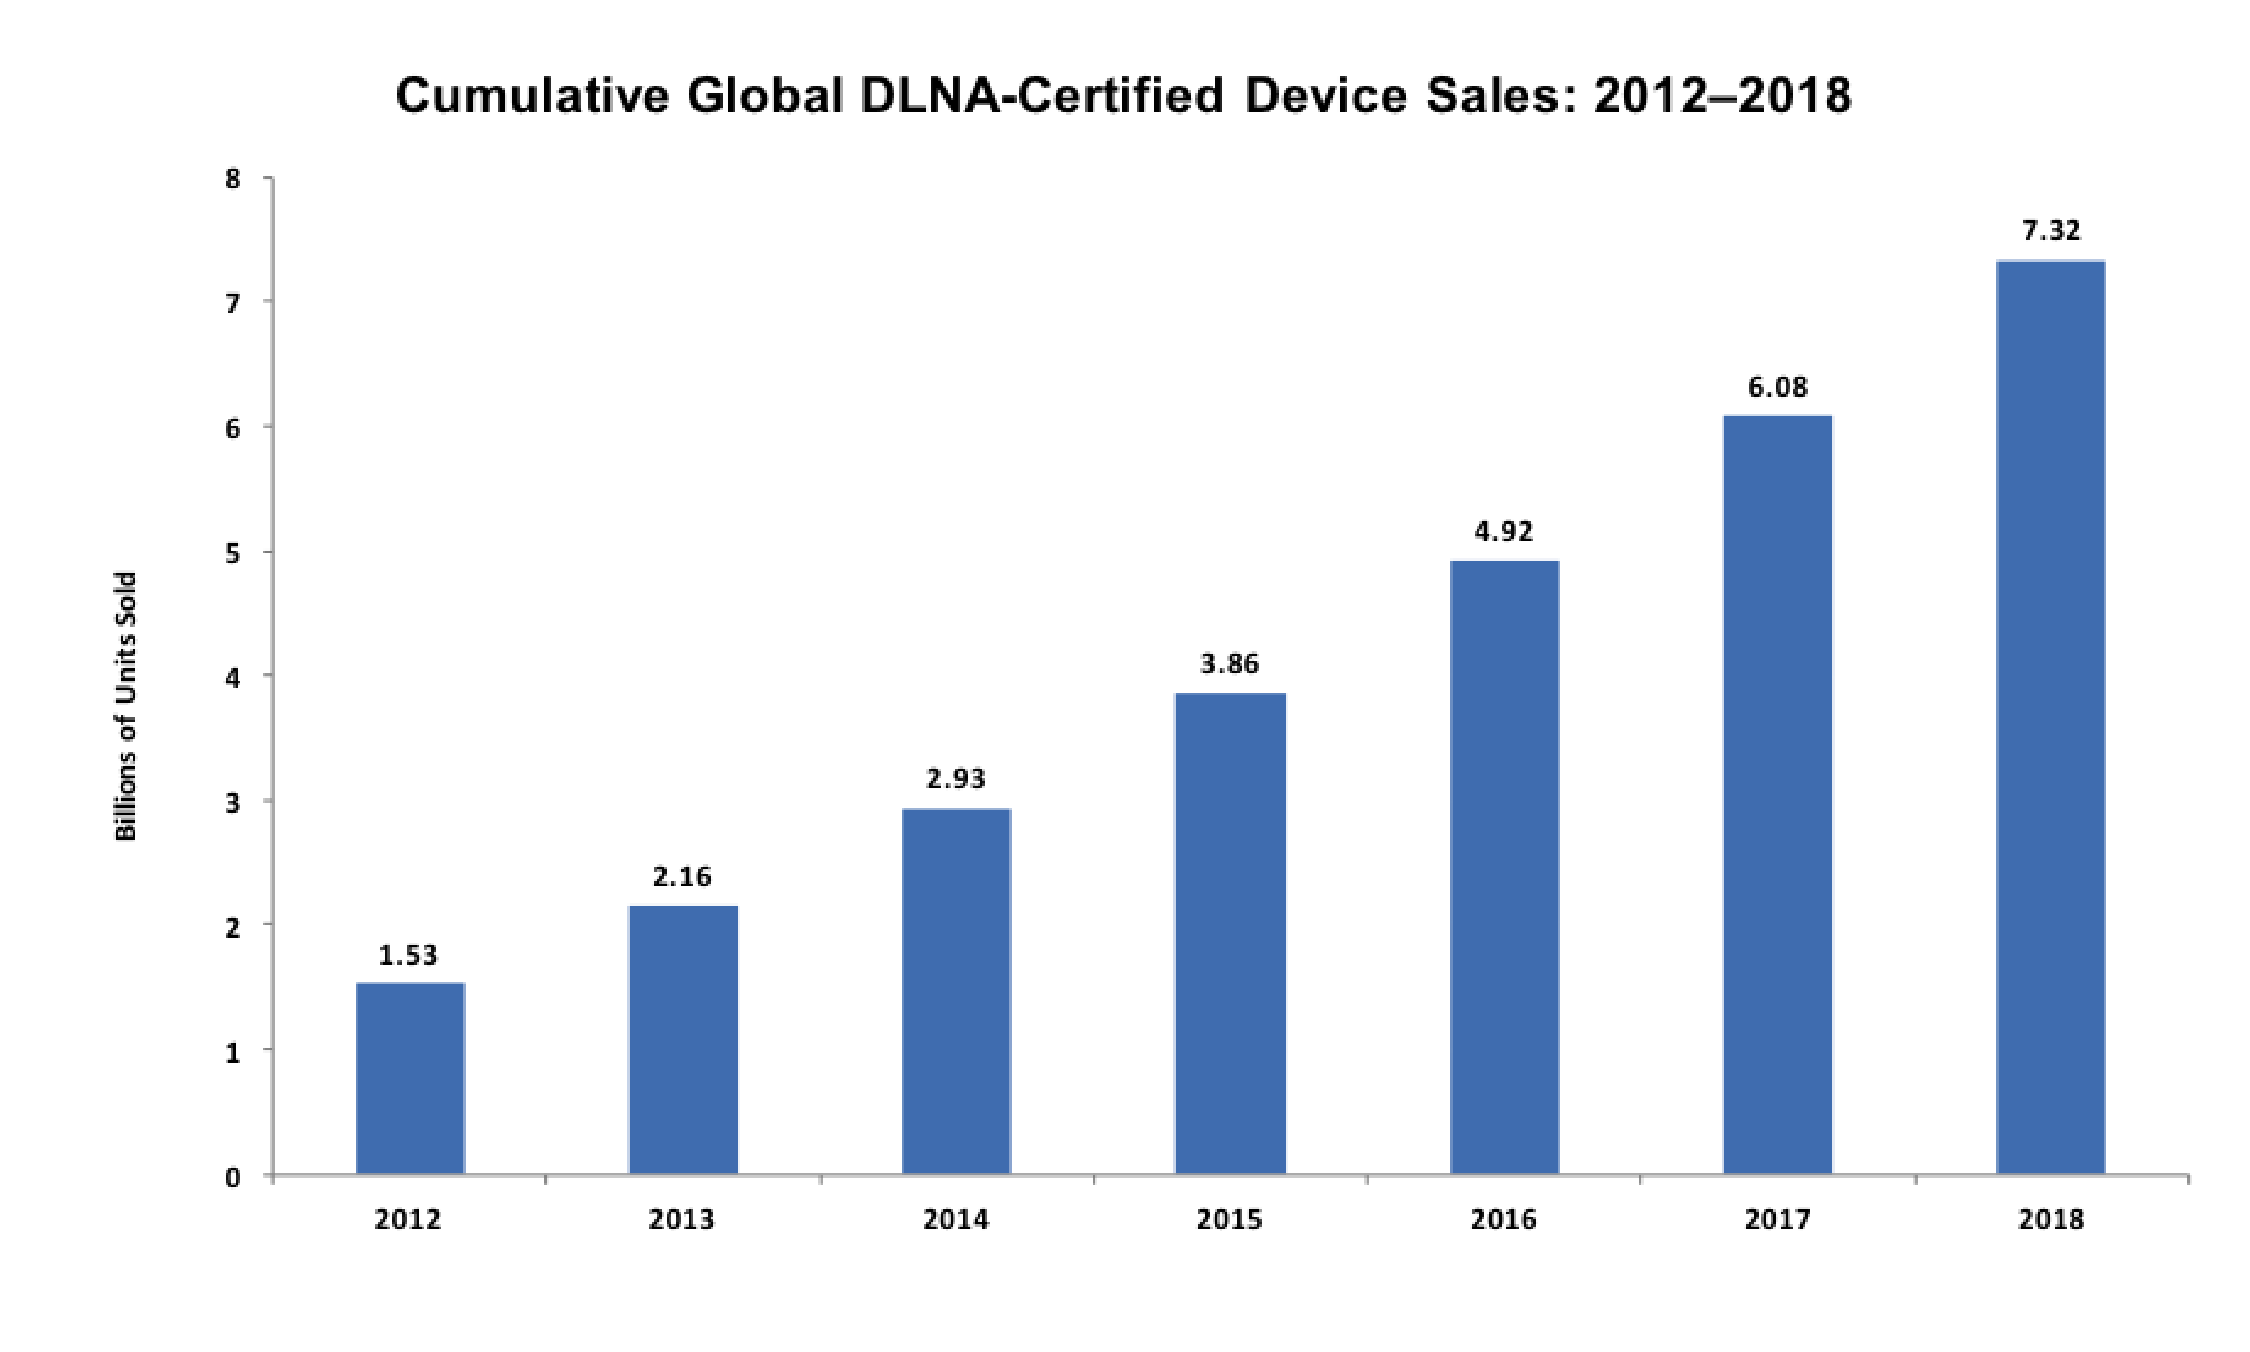
\includegraphics[height=9cm]{charts/dlna_market} 
\caption{Cumulative Global DLNA-Certified Device sales \label{dlna_market}} 
\end{figure} 

\item[--]AirPlay is bundled with Apple products, with great sales of Apple TV, Airport Express, 
Mac, iPhone, iPad, iPod, many family has just use Apple's product for 
everything. Thus AirPlay becomes the easiest way to build home networking solution, and maybe the only solution for those 
Apple users, since a lot of speaker manufactures implement their own AirPlay 
receiver on their AirPlay compatible speakers. And indeed it provides enough easy to use features to fulfill daily usage. 
\item[--]Since bundled with Android operating system, Miracast has experienced a fast growth in 
the past two years, many TVs built in the Miracast support to accept peer-to-peer Wi-Fi direct connection. 
\item[--]Chromecast dongle is a cheap device that everyone wants to try. It can easily upgrade 
old TV to "Smart TV", and since Google has provided good content support for it, it is soon accepted 
by huge amount of users. Except for Google play online sales, it also ranked top 3 best selling devices 
recently. 
\end{itemize} 

\subsubsection{Technology feature} 
\begin{enumerate} 
\item Meida format support \\ 
AirPlay and Chromecast has very limited media format support since there are 
only limited device types, so far Chromecast has only 2 device released. Apple 
TV now has 3rd generation box, but the media format support has not changed so 
much, the main improvement is the 1080p high resolution video support. On the 
other hand, DLNA has specified mandatory media formats in its specification, 
the "must have" formats only include MP3 and LPCM for music, JPEG for images and MP4 for video. 
Since Miracast is a screen mirroring technology, all formats can be played on device can be streamed. 

\item Networking technologies used \\ 

A short technology specification comparison is made to help better understanding 
the existing solutions, table \ref{Table1} below shows the main technology used 
for different popular solutions. 
%% table 1, compare technology 
\begin{table}[htb] 
\caption{Technology used comparison\label{Table1}} 
\begin{center} 
\fbox{ 
\begin{tabular}{c|l|l|l}  
\textbf{ } & Device discovery & Control Protocol & Streaming protocol \\ \hline 
\textbf{DLNA} & SSDP & UPnP & HTTP \\ \hline 
\textbf{AirPlay} & Multicast DNS & HTTP & HTTP/RTSP \\ \hline 
\textbf{DIAL} & SSDP & Chromecast & HTTP \\ \hline 
\textbf{Miracast} & Wi-Fi direct &  & Wi-Fi direct 
\end{tabular} 
} 
\end{center} 
\end{table} 

Apart from those basic technological details, some standards also offer advanced 
features compared to other solutions. For example, screen mirroring is an 
interesting feature that many standards offers. Table \ref{Table2} below shows 
what advanced features each standard provides. 
%% table 2, compare advance feature 
\begin{table}[htb] 
\caption{Advanced feature comparison \label{Table2}} 
\begin{center} 
\fbox{ 
\begin{tabular}{c|l|l|l|l}  
\textbf{ } & DLNA & AirPlay & Chromecast & Miracast \\ \hline 
\textbf{Screen mirroring} & No & Yes & No & Yes \\ \hline 
\textbf{Multiple connection} & Yes & No & No & No \\ \hline 
\textbf{Authentication} & No & Yes & No & Yes 
\end{tabular} 
} 
\end{center} 
\end{table} 


\end{enumerate} 

According to the comparison, each standard have its own features and uses 
different protocols to communicate. But there are common features supported by 
most standards, such as HTTP media server is used quite much to handle video 
and photo streaming. UPnP device discovery protocol SSDP is used quite a lot 
for device discovery. 

Since there is some similarity that is used by most standards, there is 
possibility to make an application that include all these standard 
architecture and work with those protocols. 
Making a mobile application to connect those devices becomes a doable work.
